\documentclass[9pt]{beamer}

\usepackage[utf8x]{inputenc}

\usetheme{Ampang}
%%% XeLaTeX engine for Ubuntu Font support
\usepackage{xltxtra}
\usepackage{tikz}
\setsansfont[
BoldFont=Ubuntu-Bold.ttf,
ItalicFont=Ubuntu-Italic.ttf,
BoldItalicFont=Ubuntu-BoldItalic.ttf
]
{Ubuntu-Regular.ttf}
\setmonofont{UbuntuMono-Regular.ttf}


\title{ROPER:\\A Genetic ROP-Chain Compiler Targetting Embedded Devices}
\author{Olivia Lucca Fraser}

\institute{NIMS Lab, Dalhousie University}

\begin{document}

\maketitle

\begin{frame}
\begin{center}    
    {\huge Progress Report \# 7}
    \vspace{.3cm}
    \end{center} 
\end{frame}



\begin{frame}{\theframenumber. Overview of Recent Results}
  \tikz[remember picture,overlay]
  \node[opacity=0.2, inner sep=0pt] at (current page.center)
       {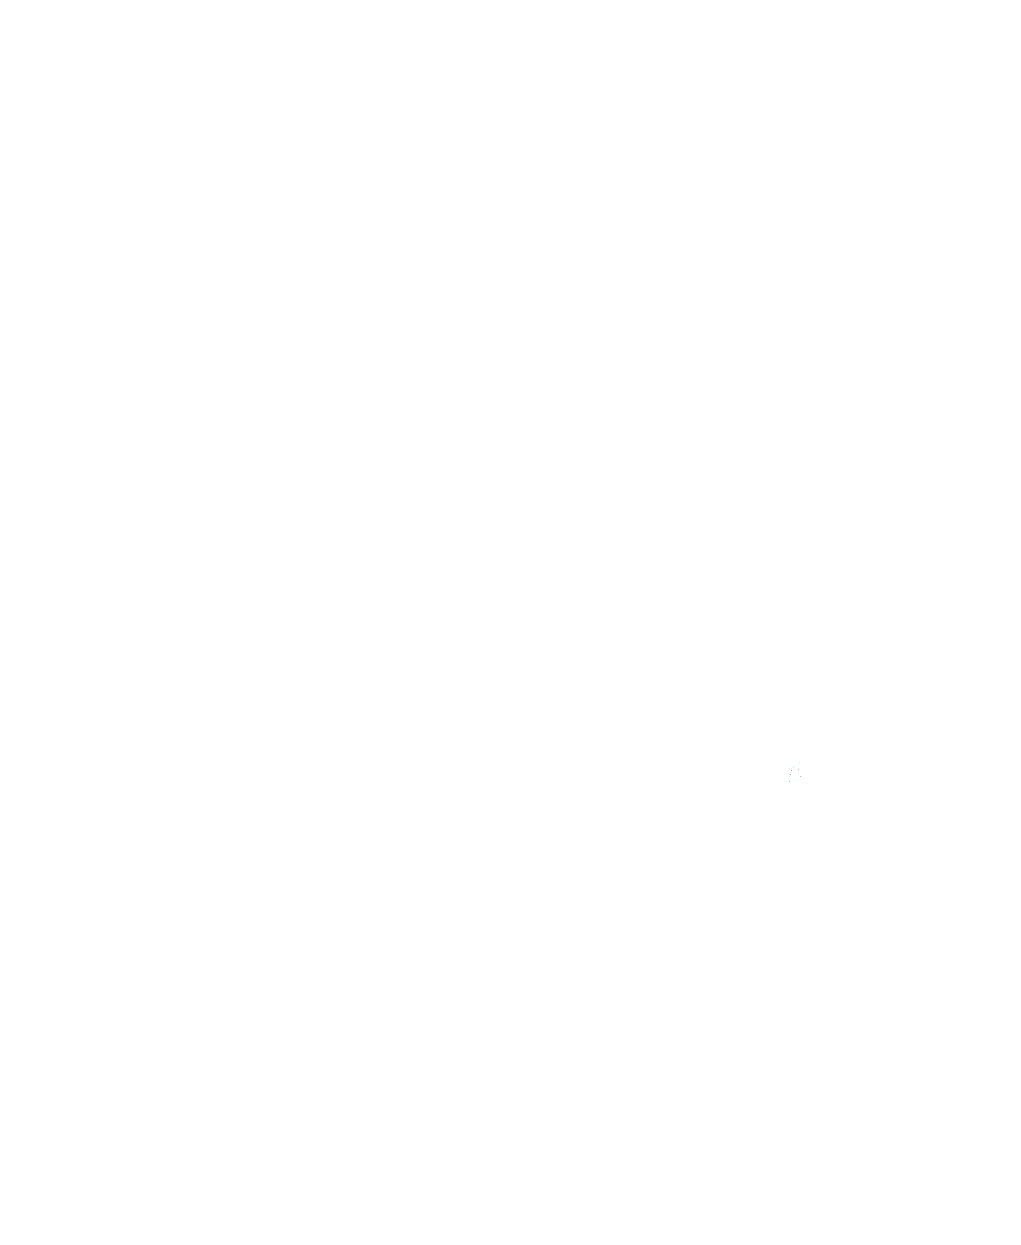
\includegraphics[width=\paperwidth,height=\paperheight]{../images/iris3.png}};
       \clearpage
  \begin{columns}
    \begin{column}{.5\textwidth}
      %\begin{itemize}

      In our last meeting, we saw how ROPER can evolve ROP-chains that perform a variety of tasks. Most interestingly, it can breed chains that exhibit learned or adaptive behaviour, and can solve a traditional benchmark classification problem: the classification of Iris specimens into species by petal and sepal measurements. 
      \vspace{8pt}

      It's important to remember that this is just an example of ROPER's capabilities. What it shows is that it is possible, in principle, to automatically generate ROP-chain payloads that behave in an adaptive and `intelligent' fashion.
      %\end{itemize}
    \end{column}
    \begin{column}{.5\textwidth}
      Here, we'll be looking more closely at a particular method for encouraging population diversity and accelerating our populations' search for optimal solutions. Unless otherwise noted, we'll be focussing on the Iris classification task reviewed in our last meeting, but the principles are general, should be applicable to virtually any problem space on which ROPER is deployed.  
    \end{column}
    \end{columns}
\end{frame}


\begin{frame}{\theframenumber. Low Hanging Fruit \& its Consequences for Diversity}
  \begin{columns}
    \begin{column}{.5\textwidth}
      \begin{itemize}
      \item A challenge facing any machine learning technique is to
      avoid getting trapped in merely \emph{local} optima.

      \item This can happen, for example, if
        it hyperspecializes on a particularly simple portion 
        -- the ``low hanging fruit'' -- of the problem set,
        while failing to adapt to more difficult problems.

      \end{itemize}
    \end{column}
    \begin{column}{.5\textwidth}
      \begin{itemize}
      \item The phenomenon is analogous to a natural population
        over-adapting to a particularly hospitable niche.
      \item But in the wild, this is
        offset by an increase in competition and crowding,
        which increase the selective pressure acting on formerly
        hospitable niches. Low-hanging fruit doesn't last very long.
      \end{itemize}
    \end{column}
    \end{columns}
\end{frame}



\begin{frame}{\theframenumber. Implementing Niching through Fitness Sharing}
  \begin{columns}
    \begin{column}{.5\textwidth}
      \begin{itemize}
      \item In order to address this issue, we first need to keep track of where, in the problem space, the overfitting occurs. Where is the low-hanging fruit?
      \item To do this, we tag each problem in our space with a `difficulty' field, which keeps track of how our specimens perform on it, on average. 
      \end{itemize}
    \end{column}
    \begin{column}{.5\textwidth}
      \begin{itemize}
      \item Since the whole point of tracking difficulty is to have it transform dynamically over the course of the evolution, we'll update these scores every so many iterations.
      \item On the next slide, we plot the progress of the population's best and average fitness scores on the left, and the difficulty rations of our problems on the right -- plotted by class mean and standard deviation. 
      \end{itemize}

    \end{column}
    \end{columns}
\end{frame}

\begin{frame}{\theframenumber. Tracking Niches without Crowding}
  \begin{center}
    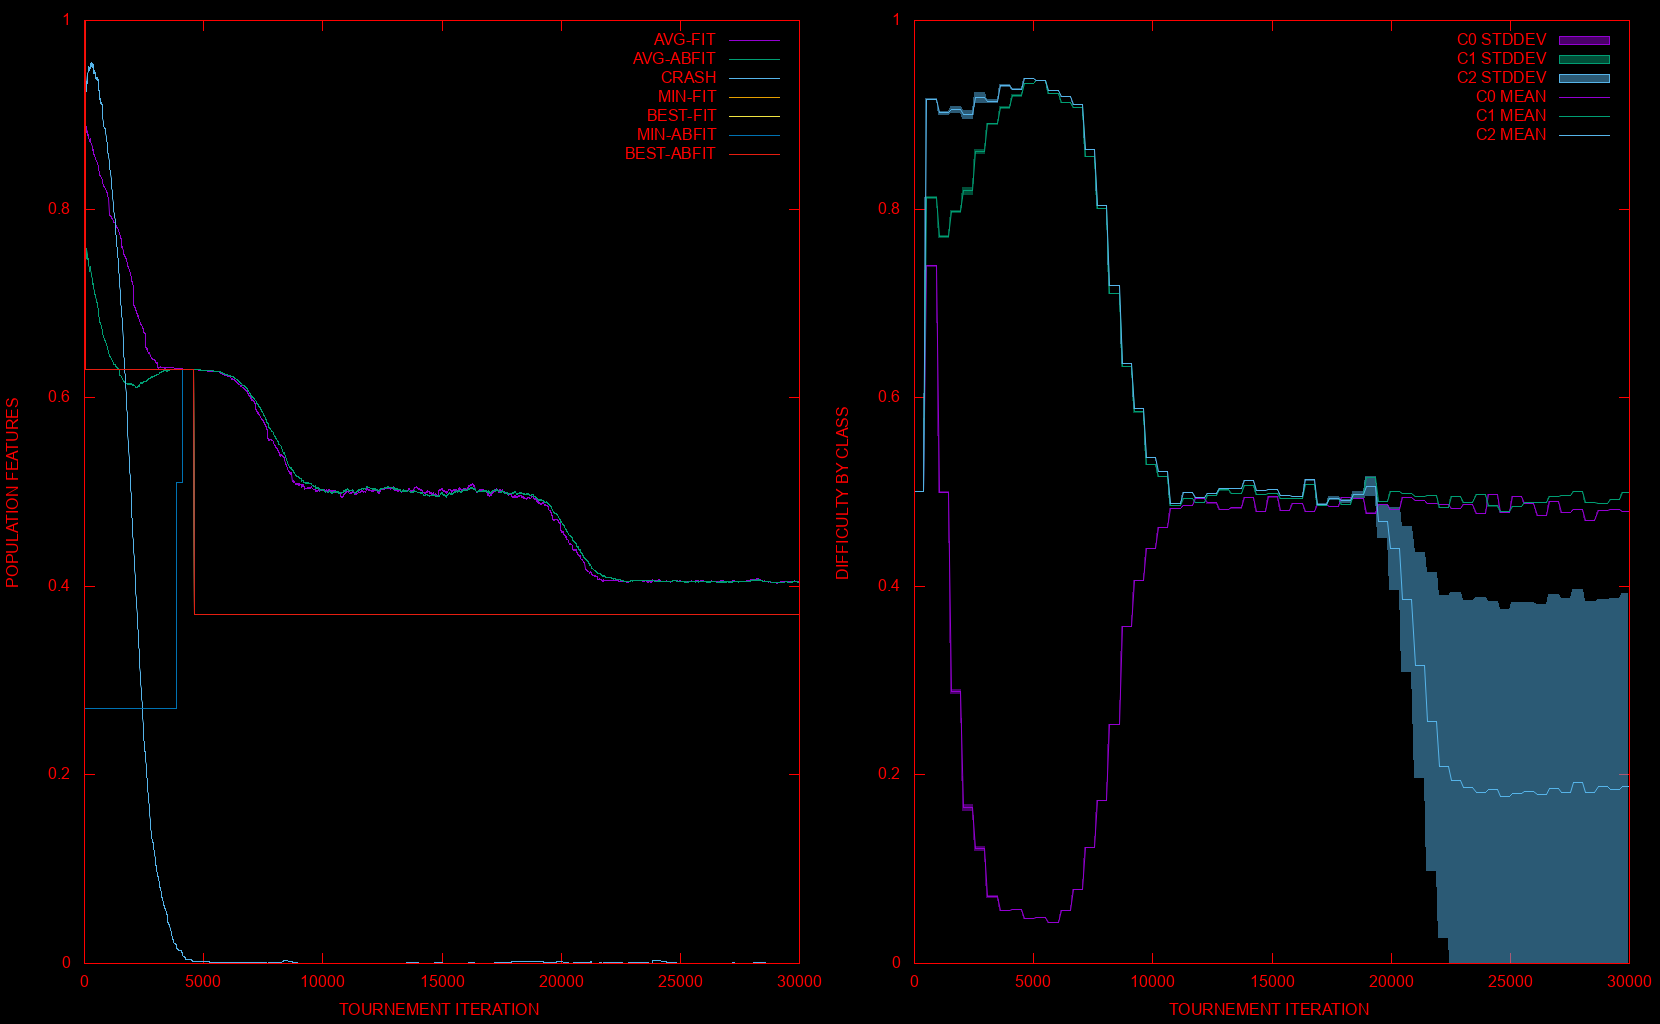
\includegraphics[width=\textwidth, height=.85\textheight]{../../examples/iris/nosharing-diff/nosharing.png}
  \end{center}
\end{frame}

\begin{frame}{\theframenumber. Crowding Implemented as Fitness Sharing}
  \begin{columns}
    \begin{column}{.5\textwidth}
      \begin{itemize}
      \item We haven't yet changed anything in the way each specimen's fitness is evaluated. The graph only shows us how the population is performing, with respect to each class of problems.
      \item But we can use this information to tweak our fitness function in ways relevant to niching.
      \end{itemize}
    \end{column}
    \begin{column}{.5\textwidth}
      \begin{itemize}
      \item All that we need to do is to scale the fitness points awareded for each problem with respect to that problem's difficulty. The rewards for solving `difficult' problems (uncrowded niches) will be greater than those awarded for solving `easy' problems (crowded niches). 
      \end{itemize}
    \end{column}
    \end{columns}

\end{frame}

\begin{frame}{\theframenumber. Niching with Crowding}
  \begin{center}
  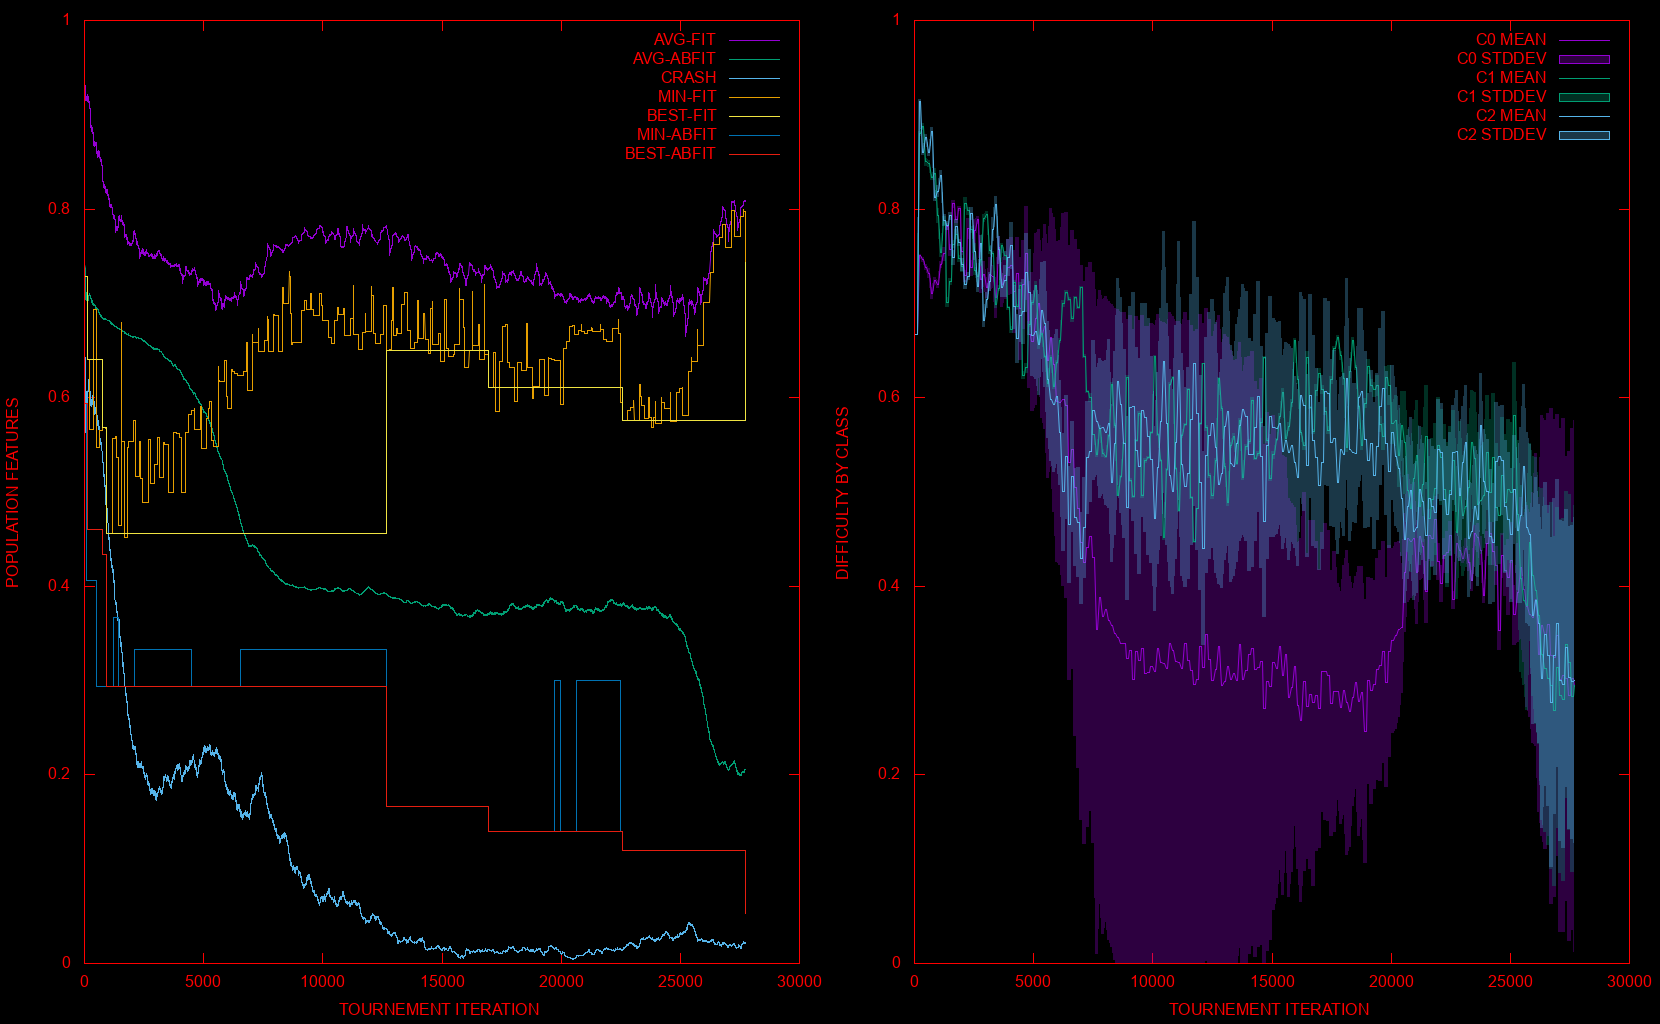
\includegraphics[width=\textwidth, height=.85\textheight]{../../examples/iris/sharing3/sharing3-black.png}
  \end{center}
\end{frame}

\begin{frame}{\theframenumber. Dynamic Braiding of Difficulty by Niche}
  \begin{figure}
    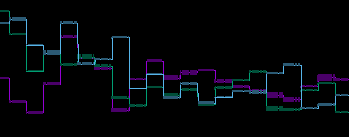
\includegraphics[width=\textwidth]{../images/braiding.png}
  \end{figure}
  A detailed view of the intricate braiding of niche availability that takes place once we enable fitness sharing. The image is an enlargement of the right panel of the graph on the last slide, focussing on the region between iterations 3000 and 5000.
\vspace{8pt}

  Because the environment perennially adjusts to the population's strengths and weaknesses, no specimen encounters the exact same fitness space as its distant ancestors, and cannot benefit from overfitting, or a diet of exclusively low-hanging fruit.
\end{frame}

\begin{frame}{\theframenumber. The Next Step}
  \begin{columns}
    \begin{column}{.3\textwidth}
      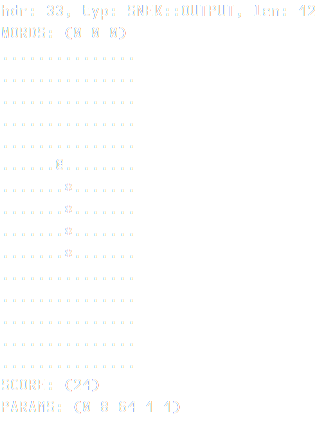
\includegraphics[height=.75\textheight]{../images/snek.png}
    \end{column}
    \begin{column}{.7\textwidth}
      I am currently working to train ROPER to handle dynamic problem spaces, beginning with simple games, like Snake and Pong. These are ideal candidates because the relevant features of the game state can be fully represented with just a small number of variables, and similarly low-dimensional controls can be sent back to the game.
      \vspace{8pt}

      The first step, already complete, is to set up an interface for ROPER and the game to communicate, over a TCP channel. For the duration of each game, the game sends packets of information to ROPER, representing its game state. The active chain processes this state information, and returns a direction for the game. The cycle repeats until the game is finished.

    \end{column}
  \end{columns}
\end{frame}



\end{document}

%%%%%%%%%%%%%%
%% TEMPLATE
%%%%%%%%%%%%%%
%% \begin{frame}{\theframenumber. }
%%   \begin{columns}
%%     \begin{column}{.5\textwidth}

%%     \end{column}
%%     \begin{column}{.5\textwidth}

%%     \end{column}
%%     \end{columns}

%% \end{frame}
